\documentclass{article}


\usepackage{arxiv}

\usepackage[utf8]{inputenc} % allow utf-8 input
\usepackage[T1]{fontenc}    % use 8-bit T1 fonts
\usepackage{hyperref}       % hyperlinks
\usepackage{url}            % simple URL typesetting
\usepackage{booktabs}       % professional-quality tables
\usepackage{amsfonts}       % blackboard math symbols
\usepackage{nicefrac}       % compact symbols for 1/2, etc.
\usepackage{microtype}      % microtypography
\usepackage{lipsum}
\usepackage{graphicx}
\usepackage{caption}
\usepackage{subcaption}
% \graphicspath{ {./images/} }
\usepackage{mathtools,amssymb}
\usepackage{tablefootnote}

\usepackage{float}
\floatstyle{plaintop}
\restylefloat{table}

\title{Solving Weighted Sokoban by A* Graph Search \\
{\sl \Large IFN680 Assignment 1}}


\author{
 Zhipeng He \\
  School of Information Systems\\
  Queensland University of Technology\\
  \textit{n10599070} \\
  \texttt{zhipeng.he@connect.qut.edu.au} \\
}


\begin{document}
\maketitle


\section{Introduction}
Sokoban is a popular puzzle game created by Hiroyuki Imabayash in 1981. In this game, the player, as a warehouse worker, must push all the boxes into a collection of storage locations (targets) by four directions (Up, Down, Left and Right) successfully without any blocks by walls or boxes. Constantly, the solution of a warehouse in this game is not unique. Some variants of sokoban games add extra rules to limit the total costs of moving, and the player can only win when finding the shortest path. This project is based on the idea of these variants and also assigns each box with a weight, which represents the cost of pushing this box. In order to achieve the success of the sokoban, it requires to find the {\it optimal solution with lowest path costs}. 

\section{Approaches}

\subsection{Algorithm}

From related works~\cite{venkatesan2018ai}, a set of search algorithms can be applied to solve the traditional sokoban puzzle, including \textit{deep first search, breadth first search, uniform cost search, A* search}, etc. For the variant of sokoban in this report, the primary task is to find the path of lowest costs to complete a warehouse, rather than solving a warehouse by any solutions. According to \cite{AIAMA}, in an ideal condition, A* search algorithm is a complete and optimal approach for minimizing the total solution cost. Consequently, A* search is chosen as the fundamental method for the sokoban solver.


\paragraph{A* graph search}

A* search is a type of best-first search algorithm, which guides search to the right path by calculating the sum~$f(n)$ of current path cost~$g(n)$ and estimated path cost~$h(n)$ to the target for each node (shown in Equ.~\ref{Astar}). 

\begin{equation}
f(n)=g(n)+h(n)
\label{Astar}
\end{equation}

So as to achieve the minimization of total solution cost, A* search always tries to find the node with lowest value of $g(n)+h(n)$ firstly and expend it to child nodes then. As the previous mentioned, the optimal A* search needs an ideal condition or requirement --- $h(n)$ must be an \textbf{admissible} heuristic or an \textbf{consistent} heuristic. For sokoban puzzle, the optimality of the heuristic should be admissible and consistent. Generally, ``the tree-search version of A* is optimal if~$h(n)$ is admissible, while the graph-search version is optimal if~$h(n)$ is consistent''~\cite{AIAMA}. As a consequence, A* graph search are used for implementing the solver. 

\paragraph{Heuristic} Considering that worker in the sokoban game can only move in four directions, some actions, like moving through diagonal, are impossible. Hence, \textit{Euclidean distance} in Equ.~\ref{Edist}, which calculates the diagonal distance between two point, might be not suitable for solving sokoban. 

\begin{equation}
    E_{dist} = \sqrt{(q_1-p_1)^2 + (q_2 - p_2)^2}
    \label{Edist}
\end{equation}

\textit{Manhattan distance}, also known as \textit{taxicab geometry}, shows the distance from $P(p_1,p_2)$ to $Q(q_1, q_2)$ in Equ.~\ref{Mdist}, which represents the sum of the absolute differences of their Cartesian coordinates. Comparing with Euclidean distance, Manhattan distance can perfectly match the path of worker in the warehouse (shown in Fig.~\ref{fig:distance}).
\begin{equation}
M_{dist} = |q_1 - p_1| + |q_2 - p_2|
\label{Mdist}
\end{equation}

\begin{figure} % picture
    \centering
    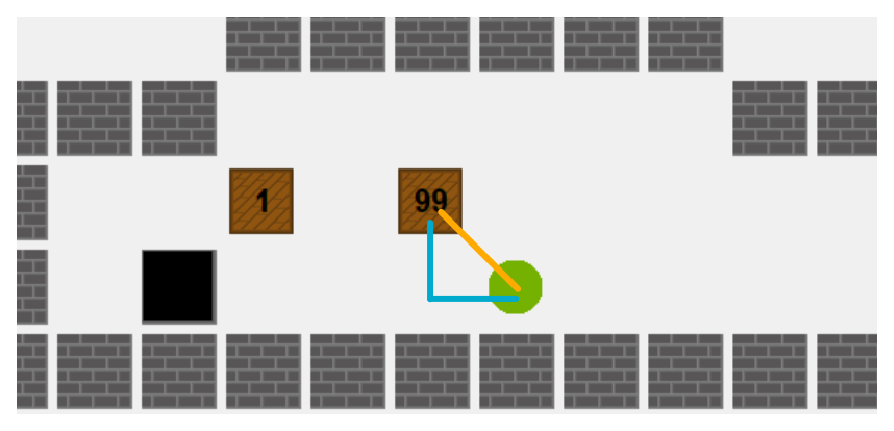
\includegraphics[width=0.5\textwidth]{image/distance.eps}
    \caption{An example of Euclidean distance (orange) and Manhattan distance (blue).}
    \label{fig:distance}
\end{figure}

For estimating the optimal value of $h(n)$, it is easy to calculate the Manhattan distance for only one box. However, sokoban warehouses may have more than one box for pushing, and a method for combining Manhattan distance for multiple boxes is required here. In this project, the heuristic function will apply \textit{Simple Lower Bound} method~\cite{master} for warehouses having more than one box, which computes and returns the sum of Manhattan distance between each box to the nearest target. In addition, the sokoban warehouses in this project also assign boxes with weights, which means the heuristic function needs to take the weight differences for boxes into consideration. 

Based on these requirements, if a warehouse has the number of $n$ box(es) and target(s), my proposed heuristic function is that: 

\begin{equation}
    h(n)= \sum^n_{i=1} \left[ {(|{b_i}_1 - {p}_1| + |{b_i}_2 - {p}_2|) \times c} +  \min_{j\in [1,\dots,n]} {(|{b_i}_1 - {t_j}_1| + |{b_i}_2 - {t_j}_2|)\times (w_i + c)} \right],
\end{equation}

where $p$ and $c$ represent the of player's coordinate position and the path cost of each movement, $i,j \in[1,\dots,n]$ are the index of box $b_i$, box weight $w_i$ and target $t_j$.


\subsection{State and problem instance}

When implementing A* graph search algorithm, the heuristic function $h(n)$ takes node $n$ as the input and only depends on the \textit{state} of that node \cite{AIAMA}. It indicates that the choice of state would take a important role in building the solver of sokoban. In this project, a sokoban warehouse is represented by a number of characters, and it is unrealistic to consider the whole warehouse as the state of node in search algorithm. Because not each part of sokoban warehouse would be modified in the progress of searching. As a result, the nodes in A* search only require dynamic features in the state. For all the static features, they should be saved in a persistent problem instance.

A sokoban is consisted of several types of cells, such as empty spaces, worker, boxes, etc. Despite the cells of free space always change when worker moves or push a box, they will not be taken into account here. Apart from the free spaces, a warehouse of sokoban can be devided into five major features, which are:

\begin{itemize}
    \item location coordinates for all wall cells (static),
    \item location coordinates for all target cells (static),
    \item location coordinates for all box cells (dynamic),
    \item location coordinates for the worker (dynamic),
    \item value of weights for each box (static).
\end{itemize}

\paragraph{State}

The positions of the worker and all boxes will be treated as the state in each node of A* star graph search algorithm. When implementing the sokoban solver, the initial state of the warehouse \texttt{self.initial} is represented by a tuple \texttt{(self.warehouse.worker, tuple(self.warehouse.boxes))}. The follow-up states share the same structure with the initial state.

\paragraph{Problem instance}

The positions of all wall and targets and the weights of boxes will be stored in the problem instance. In the implementation, they are represented by \texttt{self.walls}, \texttt{self.goal} and \texttt{self.weights} respectively. They will not change during the game.

\section{Evaluation}

\subsection{Tasks}

Three main tasks of the assignment will be solved in this project: \texttt{taboo\_cells()} function, in which finds all taboo cells (simple deadlocks) in a warehouse; \texttt{check\_elem\_action\_seq()} function, in which checks if a given sequence of actions in the warehouse is legal or not; \texttt{solve\_weighted\_sokoban()} function, in which analyses the given warehouse and finds the solution with optimisation of path and cost. 

\paragraph{Task 1: find taboo cells}

Besides the function \texttt{taboo\_cells()}, some extra functions are also be used for search all the taboo cells in the experiment. The two rules of checking taboo cells are implemented into two inner nested functions \texttt{\_rule\_1()} and \texttt{\_rule\_2()} in \texttt{taboo\_cells()}. These inner functions also call a set of auxiliary functions, such as \texttt{\_move\_in\_2d\_coordinate()}, in which calculates the final location in the 2D coordinate after a moving transformation; \texttt{\_check\_wall()}, in which checks if a cell having wall marks in the up, down, left and right of itself; \texttt{\_check\_corner()}, in which checks if a cell is a corner of the warehouse.

\paragraph{Task 2: validate action sequences}

Function \texttt{check\_elem\_action\_seq()} is the main function for checking if a given sequence is legal or not, and function \texttt{\_move\_in\_2d\_coordinate()} is also applied for calculating the movement.

\paragraph{Task 3: solve weighted sokoban}

In order to solve the weighted sokoban, function \texttt{solve\_weighted\_sokoban()} will be as the interface that creates the problem instance \texttt{SokobanPuzzle(warehouse)}, calls the search algorithm function \texttt{search.astar\_graph\_search()} and returns the solution of sequence and cost for current warehouse.

\subsection{Test Methodology}

The test designs of this project is corresponding to the previous three tasks. Here is the test methodology for each task respectively in detail.

\paragraph{Test design for task 1} 
The method for testing \texttt{taboo\_cells()} is based on the test function \texttt{test\_taboo\_cells()} in \texttt{sanity\_check.py} and creates extra test cases from warehouses, which contains rule 1 taboo cells and rule 2 taboo cells. 

\paragraph{Test design for task 2} 
Similar with task 1 design, the test function \texttt{test\_check\_elem\_action\_seq()} is also from \texttt{sanity\_check.py}. Then, some legal and illegal action sequences are created for testing.

\paragraph{Test design for task 3} 
Function \texttt{solve\_weighted\_sokoban()} is the focus of overall testing. The whole test for task 3 are combined with three steps, which are:

\begin{enumerate}
    \item A toy test by \texttt{sanity\_check.py} with example warehouses on assignment description for ensuring no syntax and functional errors.
    \item A benchmark on all given warehouse by function \texttt{test\_solve\_weighted\_sokoban\_all()}, which can automatically timeout the test longer than 5 minutes and record the names of unfinished warehouse and the results of finished warehouse into a csv file.
\end{enumerate}

\subsection{Performance}

My sokoban solver successfully passes all the designed tests for task 1 and task 2. As Fig.~\ref{fig:test1} shown that, the solver correctly and quickly returns the answers as expected. The results show that the solver is sufficient for dealing with tasks for finding taboo cells and identifying the valid action sequences. For function \texttt{solve\_weighted\_sokoban()}, my solver passed all the phase 1 testing and some results of phase 1 testing are presented in Fig.~\ref{fig:test2}. It proves that there is no simple functional or syntax errors in my codes All the tests in Fig.~\ref{fig:test} are based on the \texttt{sanity\_check.py}.

\begin{figure}
\centering
\begin{subfigure}{.5\textwidth}
  \centering
  \includegraphics[width=0.6\linewidth]{image/Test1.png}
  \caption{Task 1 and Task 2}
  \label{fig:test1}
\end{subfigure}%
\begin{subfigure}{.5\textwidth}
  \centering
  \includegraphics[width=.5\linewidth]{image/Test2.png}
  \caption{Task 3}
  \label{fig:test2}
\end{subfigure}
\caption{A screenshot for outputs by running \texttt{sanity\_check.py}}
\label{fig:test}
\end{figure}

After finishing the functional testing on particular cases, I conduct a benchmark on all given warehouses to figure out the total number of cases the solver can handle with in five minutes. The whole benchmark takes five and a half hours to process all cases. As a result, the benchmark indicates that the implemented approach can solve 39 out of 108 warehouses in the limit of five minutes and, still, 69 out of all 108 cases cannot be solved in five minutes. Table~\ref{tab:table} presents eight examples of warehouses passing the benchmark in five minutes. It suggests that the model needs more time to solver the sokoban when increasing the number of boxes and targets. Generally, my solver works efficiently in the warehouse with only two boxes, and there might be some optimisation problems for handling multiple boxes.

\begin{table}[htp!]
\centering
\resizebox{0.7\columnwidth}{!}{
\begin{tabular}{lcccccccc}
\hline
Case & 03\_im & 09    & 33    & 47    & 49    & 71    & 103   & 155   \\ \hline
Box No.  & 2      & 2     & 3     & 2     & 3     & 2     & 4     & 11(1)\tablefootnote{The are 10 boxes already in targets, and only one box needs to be solved.} \\
Time & 0.029  & 0.013 & 72.28 & 0.496 & 180.5 & 7.632 & 115.6 & 2.576 \\
Cost & None   & 396   & 41    & 179   & 82    & 48    & 35    & 282   \\ \hline
\end{tabular}
}
\caption{Running time, number of boxes and costs for part of tests}\label{tab:table}
\end{table}

\subsection{Limitations}
Based on the architecture and test results, there are some limitations for the proposed solver:
\begin{itemize}
\item The time complexity of the proposed heuristic function is $O(n^2)$, which means this solver cannot deal with warehouse with a large amount of boxes.
\item This solver can only detect some simple static deadlocks for sokoban, such as tabbo cells in this report. However, some deadlocks happen in the process of pushing box, and my solver does not have ability of find dynamic deadlocks.
\end{itemize}

\section{Conclusion}

Sokoban is a game in which the player tries to push all the boxes in a warehouse onto goal squares. It is hard for humans and computers alike. In this report, it applied A* star graph search algorithm with Manhattan distance as the heuristic fuction to solve a weighted variant of the traditional sokoban puzzle. From the results of the evaluation, it can solve some two-boxes or three-boxes sokoban with efficiency, but it will take much more time if the warehouse is more complex.


\bibliographystyle{unsrt}  
\bibliography{references}  %%% Remove comment to use the external .bib file (using bibtex).


\end{document}
